% Copyright (c) 2021 Tobias Briones. All rights reserved.
% SPDX-License-Identifier: CC-BY-4.0
%
% This file is part of https://github.com/tobiasbriones/
% cp-unah-mm700-agricultural-soil-sampling-for-data-analysis
%
% This source code is licensed under the Creative Commons Attribution 4.0
% International License found in the LICENSE-CC file in the root directory of
% this source tree or at https://spdx.org/licenses/CC-BY-4.0

\section{Muestreo Sistemático}

Para realizar un muestreo sistemático se siguen los siguientes cálculos:

\bigbreak

Dado el tamaño de la población $N$ y el número de muestras $n$, hacer $k=\ceil{\frac{N}{n}}$. El valor $k$ es el período que hace que el muestreo sea sistemático. Tomar un punto aleatorio $K \in [1, k]$. Cada unidad dada por $K$, $K + k$, $K + 2k$, ... , etc., define la muestra.

\bigbreak

En ciertos casos el muestreo sistemático es el mismo MAS por lo que se pueden aplicar técnicas del MAS. Otras veces funciona como un intermediario (proxy) hacia el MAS ya que como se puede notar, si la población está dispuesta de forma aleatoria entonces lo que se tendría sería básicamente un MAS. También se debe tener en cuenta que la probabilidad de un grupo de ser escogido no es la misma como en el MAS. Otro uso que puede tener este tipo de muestreo es de hacer un trabajo similar al muestreo por clúster. De estos factores depende que la muestra sea representativa ya que si la población está ordenada de acuerdo a su índice entonces la muestra no servirá (p. ej. solo salen unidades del mismo tipo al estar ordenadas por posición, si hay hombres y mujeres solo salen hombres por ser posición par).

\bigbreak

\begin{figure}[H]
    \centering
    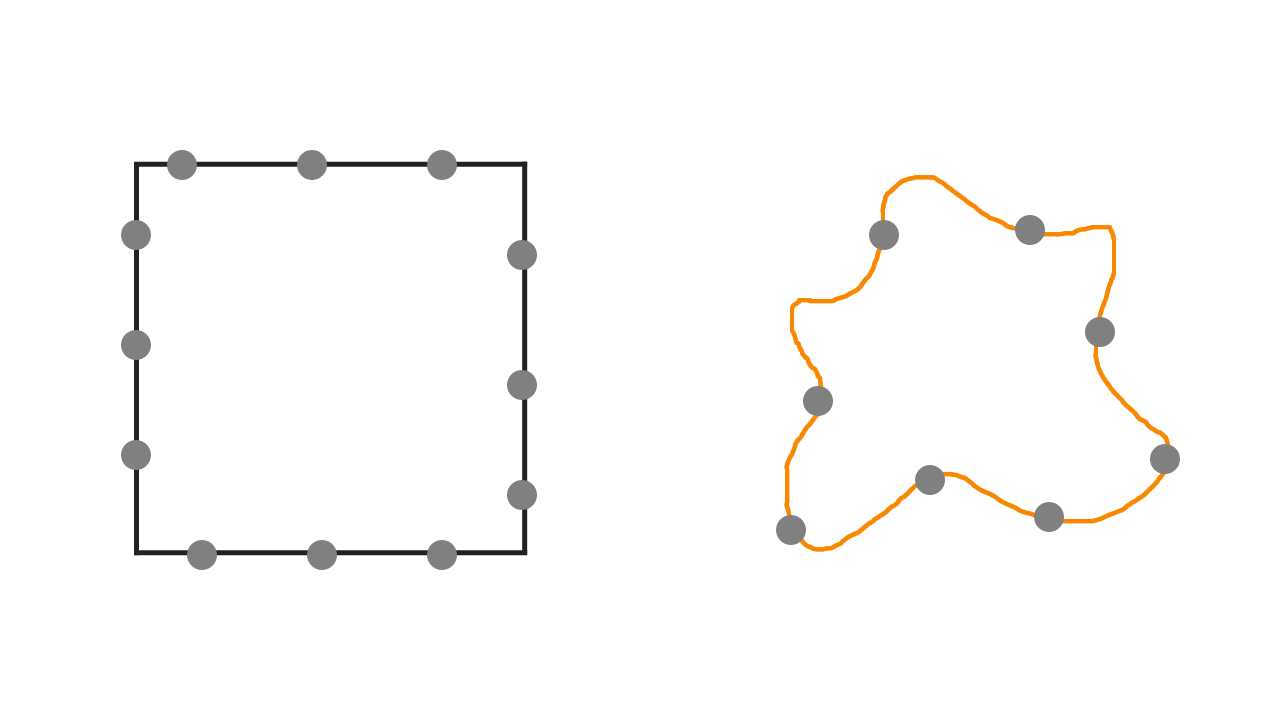
\includegraphics[width=0.3\paperwidth]{img/soil-systematic-sampling.png}
    \caption{Posible muestreo sistemático de un lote}
\end{figure}

La ilustración de arriba describe una de muchas estrategias \cite{lassaga-2011} \cite{gobpe-ministerio-del-ambiente-2014} para tomar las muestras del suelo. En este caso se toma el perímetro del suelo y sistemáticamente se toman las muestras por el perímetro, las cuales también pueden ser determinadas por otros patrones como diagonal o zigzag.

\bigbreak

Hay que tomar en cuenta que el muestreo sistemático no siempre produce una muestra representativa por lo dicho más arriba, esto es, cuando hay una distribución periódica de las unidades. Para los estudios ecológicos de suelos \cite{lohr-2009}: \say{Puede haber una topografía de crestas y surcos que daría lugar a un patrón periódico de vegetación. Si un esquema de muestreo sistemático sigue el mismo ciclo, la muestra no se comportará como una MAS}.
